% MyLocal_LLM research note 0090B; living design and evidence register.
% Build from repo root:
%   latexmk -pdf -interaction=nonstopmode -halt-on-error -output-directory=/tmp/0090b-build \
%     docs/research/0090B_modular_residual_specialist_combination.tex
% Edits: update the version/change log and distinguish reported from archived evidence.
\documentclass[11pt,letterpaper]{article}
\usepackage[T1]{fontenc}
\usepackage[utf8]{inputenc}
\usepackage{lmodern,microtype}
\usepackage[margin=0.87in,headheight=17pt]{geometry}
\usepackage{amsmath,amssymb,mathtools}
\usepackage{booktabs,tabularx,longtable,array}
\usepackage{graphicx}
\usepackage{xcolor}
\usepackage{hyperref}
\usepackage{fancyhdr}
\usepackage{enumitem}
\usepackage{listings}
\usepackage{tikz}
\usetikzlibrary{positioning,arrows.meta,fit}
\definecolor{darkblue}{HTML}{17324E}
\definecolor{sea}{HTML}{006F78}
\definecolor{slate}{HTML}{52677B}
\definecolor{pale}{HTML}{F0F5F8}
\definecolor{ink}{HTML}{202D39}
\definecolor{softorange}{HTML}{F9F1E5}
\hypersetup{colorlinks=true,linkcolor=darkblue,urlcolor=sea,citecolor=sea,
 pdfauthor={MyLocal LLM research project},
 pdftitle={Modular Residual Specialists and Learned Combination -- Living Research Note 0090B}}
\setlength{\emergencystretch}{4em}
\setlist[itemize]{leftmargin=17pt,topsep=3pt,itemsep=2pt}
\setlist[enumerate]{leftmargin=21pt,topsep=3pt,itemsep=2pt}
\pagestyle{fancy}\fancyhf{}
\fancyhead[L]{\small\color{slate} MYLOCAL\_LLM / RESEARCH NOTE 0090B}
\fancyhead[R]{\small\color{slate} 2026-10-26 / v0.1}
\fancyfoot[L]{\small\color{slate} Living architectural proposal, not a validated specialist ensemble}
\fancyfoot[R]{\small\color{slate}\thepage}
\newcommand{\vocab}{\mathcal V}
\newcommand{\R}{\mathbb R}
\newcommand{\softmax}{\operatorname{softmax}}
\newcommand{\CE}{\operatorname{CE}}
\newcommand{\KL}{D_{\mathrm{KL}}}
\newcommand{\code}[1]{\path{#1}}
\newcommand{\tagg}[1]{\textsf{\footnotesize\color{sea}\textbf{[#1]}}}
\newcommand{\infobox}[1]{\noindent\colorbox{pale}{\parbox{\dimexpr\linewidth-2\fboxsep\relax}{\small #1}}\par}
\newcommand{\TODO}[1]{\textcolor{sea}{\textbf{[OPEN: #1]}}}
\lstset{basicstyle=\ttfamily\footnotesize,breaklines=true,columns=fullflexible,
 frame=single,framesep=4pt,showstringspaces=false}
\begin{document}
\begin{center}
{\LARGE\bfseries\color{darkblue} Modular Residual Specialists\\[3pt] and Learned Combination}\par\vspace{6pt}
{\large\color{slate} Architecture, prior probability-fusion evidence, and a reproducible research roadmap}\par\vspace{10pt}
{\normalsize MyLocal\_LLM research project}\par\vspace{4pt}
{\small \textbf{Living report v0.1} \quad 26 October 2026 \quad Series 0090B}
\end{center}
\vspace{7pt}
\infobox{\textbf{Evidence boundary.} The \emph{existing} probability combiner and its measured checkpoints are distinct from the \emph{proposed} foundation-plus-specialist combiner. The first frozen-foundation / residual-specialist CPU prototype was reported under patch 0090A; a trained, multi-specialist combination has \textbf{not} been demonstrated. All cross-entropy results below concern the earlier probability-fusion experiments unless explicitly identified otherwise. Numerical results recalled from conversations are flagged separately from archived, repository-backed benchmarks.}
\begin{abstract}
The research objective is to expand a single, frozen general-language foundation with several independently trained Transformer specialists whose outputs correct its contextual predictions. A specialist need not be a small adapter: the nominal long-run target is a 12-layer, width-1024, FFN-4096 Transformer (approximately 182 million dense-block parameters), while the two-layer implementation is only a correctness probe. Each specialist may have a different causal historical-memory reader, including a longer retrievable horizon than the foundation. This note defines the mathematical interface between the foundation, specialists, and combiners; compares probability averaging, residual-logit fusion, and residual-hidden-state fusion; documents the earlier 0082-series combination results and 2026-10-25 performance measurements; and establishes controls, acceptance criteria, and a versioned evidence ledger for future experiments. The aim is to test \emph{whether domain-specific capacity can be added more efficiently and composably than retraining entire models}, not to presume that combining networks automatically yields a stronger language model.
\end{abstract}
\tableofcontents
\clearpage

\section{Scope, factual status, and design principles}
\label{sec:scope}
\subsection{What is implemented versus proposed}
\begin{tabularx}{\linewidth}{@{}p{0.25\linewidth}X p{0.16\linewidth}@{}}
\toprule
Component & Current state and important boundary & Classification \\
\midrule
Frozen general foundation & Approximately 338.1M parameters, 20 layers, width 1024, FFN 4096, vocabulary 32768; 4096-token working window and compact historical retrieval to approximately 65536 tokens. & Existing \\
Probability fusion (0082/0084) & Combines full-vocabulary distributions of separately evaluated frozen teachers; optional learned model-to-token-context weighting and unrestricted probability residual. & Implemented \\
Residual specialist (0090A) & Frozen foundation $H_0$ feeding trainable Transformer blocks; zero-initialized correction uses frozen $W_U$. CPU tests reported; RTX production validation pending. & Prototype \\
Specialist ensemble combiner & Jointly uses the foundation, independently trained residual specialists, and a reliability/gating mechanism. & \textbf{Proposal} \\
Per-specialist private history & Each specialist may independently retrieve more, fewer, or different historical blocks than the foundation. & \textbf{Proposal} \\
Sparse routing & Execute only selected specialists after a foundation-only pre-routing decision. & \textbf{Proposal} \\
\bottomrule
\end{tabularx}

\subsection{Non-negotiable research constraints}
\begin{itemize}
\item \textbf{Foundation preservation:} frozen foundation parameters, vocabulary head and tokenizer; no accidental gradients or optimizer updates.
\item \textbf{Independent specialists:} checkpoints and training tasks are separable; a specialist must not require retraining unrelated specialists.
\item \textbf{Configurable depth and memory:} two layers for integration; approximately 12 layers at width 1024 is the anticipated research size. Historical capacity belongs to each specialist's configuration, not an immutable property of the foundation.
\item \textbf{Strict causality:} all gates, representations, and retrieval candidates at target $t$ are functions only of tokens available before that target. Whole-document leakage and mislabeled source positions are disallowed.
\item \textbf{Realistic compute:} RTX 5080 (16 GiB), roughly 64 GiB host RAM, CuPy/BF16, frozen-model forward only, chunked output head, CPU optimizer-state offload, and no padded full-history attention.
\item \textbf{Measurable value:} the combined system must improve disjoint held-out data and ideally executable domain tasks \emph{relative to its strongest constituent}, at a documented training/inference cost.
\end{itemize}

\section{Architecture and information contract}
\label{sec:architecture}
Let $x_{\le t}$ be the causal input prefix. The frozen foundation returns a sequence of \emph{normalized} contextual hidden states $H_0\in\R^{T\times d_0}$, $d_0=1024$, and the frozen vocabulary projection $W_U\in\R^{d_0\times V}$. Its baseline logits and probabilities at a scored position are
\begin{equation}
 z_0=H_0 W_U,\qquad p_0=\softmax(z_0),\qquad V=32768.
 \label{eq:foundation}
\end{equation}
A specialist $i$ receives at minimum $H_0$, optionally token embeddings $E(x)$ and an independently defined causal historical source view $\mathcal M_i(x_{\le t})$. It predicts a \emph{hidden residual}, not a separate vocabulary model:
\begin{equation}
 \Delta H_i=S_i\bigl(H_0,\,E(x)\;\text{(optional)},\,\mathcal M_i\;\text{(optional)}\bigr),\quad
 \Delta z_i=\Delta H_iW_U,\quad z_i=z_0+\Delta z_i.
 \label{eq:individual}
\end{equation}
A specialist run by itself uses $p_i=\softmax(z_i)$. Its correction output is initially zero so the initial standalone specialist matches the foundation exactly. The residual is added \emph{after} the foundation's final normalization; a new post-addition normalization would alter the intended identity and the fusion algebra.

\begin{figure}[h]
\centering
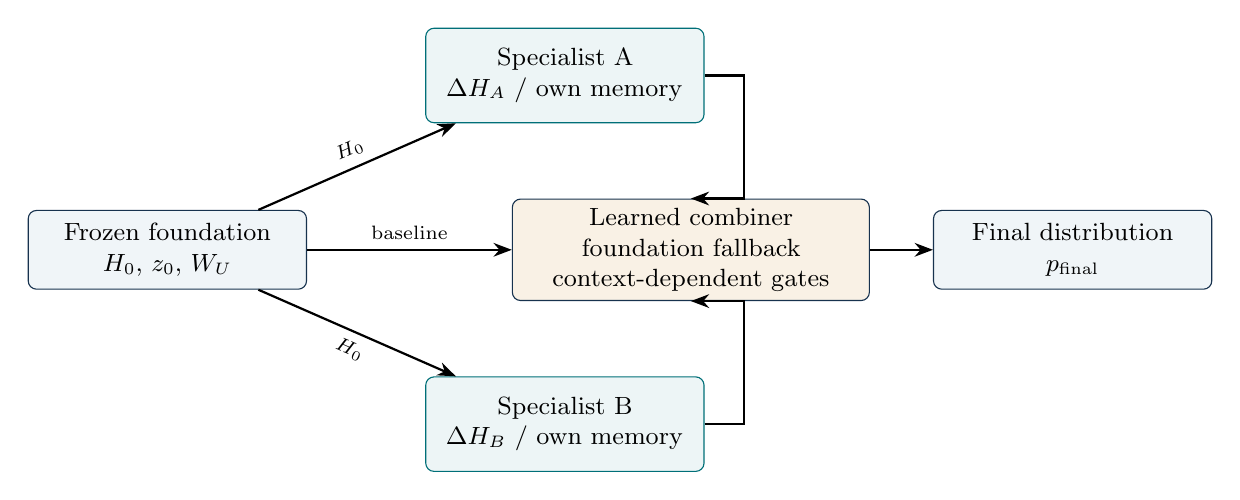
\begin{tikzpicture}[>=Stealth,node distance=7mm and 8mm,
 box/.style={draw=darkblue,rounded corners=3pt,align=center,fill=pale,minimum height=10mm,text width=33mm},
 spec/.style={draw=sea,rounded corners=3pt,align=center,fill=sea!7,minimum height=12mm,text width=33mm},
 gate/.style={draw=darkblue,rounded corners=3pt,align=center,fill=softorange,minimum height=12mm,text width=43mm},font=\small]
 \node[box] (base) {Frozen foundation\\$H_0$, $z_0$, $W_U$};
 \node[spec,above right=11mm and 15mm of base] (a) {Specialist A\\$\Delta H_A$ / own memory};
 \node[spec,below right=11mm and 15mm of base] (b) {Specialist B\\$\Delta H_B$ / own memory};
 \node[gate,right=26mm of base] (comb) {Learned combiner\\foundation fallback\\context-dependent gates};
 \node[box,right=8mm of comb] (out) {Final distribution\\$p_{\rm final}$};
 \draw[->,thick] (base) -- node[above,sloped,font=\scriptsize] {$H_0$} (a);
 \draw[->,thick] (base) -- node[below,sloped,font=\scriptsize] {$H_0$} (b);
 \draw[->,thick] (base) -- node[above,font=\scriptsize] {baseline} (comb);
 \draw[->,thick] (a.east) -- ++(5mm,0) |- (comb.north);
 \draw[->,thick] (b.east) -- ++(5mm,0) |- (comb.south);
 \draw[->,thick] (comb) -- (out);
\end{tikzpicture}
\caption{Logical interfaces, not a claim that all specialists must execute on every token. An eventual pre-router can gate specialist execution using foundation-only information.}
\end{figure}

\subsection{Independently configurable specialists}
The specialist registry should carry stable identities and per-specialist fields: number of layers, width, FFN width, attention schedule, working length, precision, input adapter, hidden-output adapter, expected foundation fingerprint, and a versioned memory description. A 12-layer, width-1024, FFN-4096 specialist is approximately 182M \emph{block} parameters (excluding adapters); the 2-layer configuration (approximately 30M) is a smoke test, \emph{not} the target for practical capability studies. Narrower specialists (widths 512 or 768) remain legitimate independent ablations.

\subsection{Correctness and identity invariants}
\begin{enumerate}
\item \textbf{Zero specialist identity:} if $\Delta H_i=0$ for all present specialists, every proposed combination below must return $p_0$ under its corresponding neutral gating/residual initialization.
\item \textbf{Foundation fallback:} a trained combiner must be able to choose $p_0$ (or $z_0$) without paying for a correction that is actively harmful.
\item \textbf{Permutation consistency:} reordering identical $(\mathrm{id}_i,\Delta H_i)$ pairs cannot affect output; identities themselves may legitimately affect learned reliability.
\item \textbf{Frozen-gradient isolation:} training a combiner changes neither foundation nor specialist weights; training one specialist changes neither the foundation nor any other specialist.
\item \textbf{Compatibility:} reject mismatched foundation/tokenizer fingerprints; log specialist memory configuration and effective retrieval budget.
\end{enumerate}

\section{Prior combination research: measured evidence}
\label{sec:results}
\infobox{\textbf{Source convention.} \tagg{ARCHIVED} refers to documentation or source code inside the supplied repository. \tagg{CONVERSATION} refers to results reported in prior project discussions and recovered for this handoff, for which the original CSV/log is \emph{not present} in the supplied archive. \tagg{DERIVED} is arithmetic performed on those reported values. Such numbers are preliminary unless rerun from exact immutable checkpoints on disjoint test material. These experiments involved \emph{independent frozen teacher predictions}, not trained residual specialists.}

\subsection{0082A--0082J: what the current combiner actually does}
\tagg{ARCHIVED}\; The implemented \code{mini_llm/collective/probability_fusion.py} is a model-identity-aware, full-vocabulary combiner. Each teacher supplies FP32 logits $z_i\in\R^V$; the model evaluates $p_i=\softmax(z_i)$. Uniform arithmetic and normalized geometric reference distributions can be evaluated; the learned reference is
\begin{equation}
 p_{\mathrm{ref}}(v\mid x)=\sum_{i\in\mathcal A}w_i(x)p_i(v\mid x),\quad
 w_i(x)=\softmax_{i\in\mathcal A}[a_i+\delta_i(x)],
 \label{eq:existing-ref}
\end{equation}
where $a_i$ are learned global identity logits. With context gating enabled (0082J), each identity embedding queries preceding \emph{token embeddings} through two recency-biased attention heads; a small MLP generates $\delta_i(x)$. There is no GRU context summary, no requirement to share teacher hidden widths, and no large context self-attention. At context-head count zero, the adjustment is disabled and weights are global. The final result is an \emph{unrestricted vocabulary residual applied to log reference probabilities}:
\begin{equation}
 p_{\mathrm{0082}}(v\mid x)=\softmax_v\bigl(\log p_{\mathrm{ref}}(v\mid x)+r_\phi(v,x,\{p_i\})\bigr).
 \label{eq:0082}
\end{equation}
Its final residual projection and context score projection begin at zero, preserving the corresponding simpler prediction initially. The residual decoder also uses full probability-vector information, probability-weighted vocabulary embedding moments, per-member entropy features, and model identities; it is \emph{not} equivalent to blending the specialists' hidden corrections. See the implementation and \code{docs/0084B_CORE_ONLINE_FUSION.md}.

\subsection{Early Deep+Wide experiments}
\tagg{CONVERSATION}\; Earlier Deep and Wide checkpoints were distinct model architectures. In the fixed-validation Deep+Wide evaluation discussed around 18--24 October 2026, the following were reported (same comparison target set \emph{within} this run):
\begin{center}
\begin{tabular}{@{}lr@{}}\toprule
Predictor or combination & CE (nats/token) \\
\midrule
Deep teacher (32 layers, width 512) & 4.13264 \\
Wide teacher (13 layers, width 768) & 4.04743 \\
Arithmetic probability average & 3.98138 \\
Learned global weighting, selected step 600 & 3.97915 \\
Neural probability residual, selected step 600 & \textbf{3.96573} \\
\bottomrule\end{tabular}
\end{center}
\tagg{DERIVED}\; Relative to the best teacher, arithmetic averaging contributed $0.06605$ CE improvement; adjusting the global model weights contributed a further $0.00223$, and adding the learned residual contributed $0.01342$. Total improvement was $0.08170$ nats/token. This is evidence that complementary weak teachers \emph{can} combine usefully on that selected validation set; it does not establish specialist gains or a robust out-of-distribution improvement.

\tagg{CONVERSATION}\; The same 0082I learning-history discussion reported step-wise \emph{fusion} validation CE approximately $3.98137$ initially, $3.96573$ at step 600 (selected), $3.96875$ at step 1000, $3.97714$ at step 2000, and $3.98801$ at step 3000. The degradation after step 600 makes early stopping, data separation, and residual regularization important research variables. A \emph{separate subsequent report} gave Deep $4.13264$, Wide $4.04743$, arithmetic $3.98138$, weighted $3.97879$, and fusion $3.96096$; its specific checkpoint/step is not recoverable here, so it must \emph{not} be merged with the step-600 row or treated as a further epoch of the same immutable run.

\subsection{Earlier 0082F residual experiment (distinct evaluation)}
\tagg{CONVERSATION}\; Another earlier 0082F streaming experiment reported an arithmetic reference of $3.73184$, a geometric reference of $3.71212$, and a best fusion CE of $3.70668$ at step 400, followed by deterioration. These numbers belong to \emph{another} experimental setup: no cross-run CE difference is meaningful without checking checkpoints, data split, context geometry and tokenizer.

\subsection{Two identical 338M teachers: residual-only control}
\tagg{CONVERSATION}\; In an identical-checkpoint control, both members came from the same 338M checkpoint. The reported validation CE changed from approximately $2.95617$ to $2.95539$ by step 775 (gain $0.00078$), with global weights near $0.5/0.5$. For strictly identical distributions, arithmetic, geometric and any normalized weighted mixture \emph{must equal the teacher distribution}; a nonzero gain, if reproducible, is due to learned recalibration/residual behavior, \emph{not} teacher diversity. This is a valuable control but the small validation set does not support a strong generalization claim.

\subsection{Two different-stage 338M checkpoints (October 25)}
\tagg{CONVERSATION}\; A later comparison used two different checkpoints of the same 20-layer, width-1024 model (including directories \code{0083_intermediate_20L_1024_fullmix_100k_14k} and \code{0083_intermediate_20L_1024_fullmix_100k}). The following \emph{same-target} validation scores were reported at fusion step 725:
\begin{center}
\begin{tabular}{@{}lr@{}}\toprule
Predictor or combination & CE (nats/token) \\
\midrule
Checkpoint member 0 & 2.69441 \\
Checkpoint member 1 (stronger) & 2.64526 \\
Arithmetic probability average & 2.62739 \\
Learned weighted reference & 2.62473 \\
Weighted reference + vocabulary residual & \textbf{2.62403} \\
\bottomrule\end{tabular}
\end{center}
\tagg{DERIVED}\; Against the stronger member, the arithmetic, weighting, and learned-residual increments are respectively $0.01787$, $0.00266$, and $0.00070$ nats/token; total apparent gain $0.02123$. The source discussion also reported the full fusion validation CE improving from $2.62627$ (step 250) to $2.62403$ (step 725), and global weights shifting roughly $0.47/0.53\to 0.40/0.60$. These results used only \emph{16 validation windows}, repeatedly consulted during selection, and are not a blind held-out-test guarantee. The reported weighting gain cannot be attributed specifically to 0082J context attention without a matched $\delta_i(x)\equiv0$ ablation.

\subsection{Full-vocabulary fusion GPU cost: archived benchmark}
\tagg{ARCHIVED}\; \code{docs/FUSION_OPT_01_COMPREHENSIVE_GPU_OPTIMIZATION.md} contains a dated October 25, 2026 RTX 5080 benchmark of the existing probability combiner. For the measured large configuration (member width 64, decoder width 24, depth 4, two context heads; 64 scored rows, $V=32768$), an optimization reduced median update latency from $73.14$ to $36.38$ ms, increased reported combiner throughput from $875$ to $1759$ scored tokens/s, and reduced sampled peak live CuPy allocation from $6224$ to $5456$ MiB. This is a \emph{combiner-microbenchmark}, not a full specialist-ensemble inference figure. A production-equivalent checkpoint experiment reported $1785$ combiner scored tokens/s and $1668$ end-to-end tokens/s, versus an earlier production report around $937$ tokens/s. GPU pool reservation was not reported in the standalone allocation metric; these results do not establish the memory footprint of an additional 12-layer specialist.

\subsection{Evidence interpretation and remaining uncertainty}
\begin{itemize}
\item Probability averaging can exploit diversity, even when the two individual models are weaker than the combined prediction. It says nothing by itself about whether independently trained \emph{hidden residual specialists} compose linearly.
\item Global reliability weighting and vocabulary-residual calibration show some measurable benefit. The \emph{incremental contribution of model-query context attention} remains unmeasured on a matched held-out ablation.
\item The historical 0082/0084 online teacher path deliberately disables long-history reads and evaluates plain, short local context; none of those scores is a benchmark of 64K historical retrieval or specialist-owned memory.
\item Validation checkpoint selection, small window counts, checkpoint/seed drift and source differences can inflate apparent gains. Numerical gains below $10^{-3}$ nats/token require paired uncertainty analysis and genuinely untouched evaluation data.
\item None of these measurements is evidence for a trained multi-specialist router. All observations above are priors guiding a new controlled experiment.
\end{itemize}

\section{Three distinct specialist-combination formulations}
\label{sec:alternatives}
All three formulations use the foundation and specialists defined in \eqref{eq:foundation}--\eqref{eq:individual}. Let $\mathcal A_t$ be the available specialist identities for target $t$; $0$ denotes the foundation fallback. Gates are token-dependent but must be causal and exclude non-loaded specialists.

\subsection{A. Probability mixture: conservative initial control}
\begin{equation}
 p_{\mathrm{mix}}(v\mid x_{\le t})=
 w_0(x_{\le t})p_0(v)+\sum_{i\in\mathcal A_t}w_i(x_{\le t})p_i(v),\qquad
 w_i\geq0,\quad\sum_{i\in\{0\}\cup\mathcal A_t}w_i=1.
 \label{eq:pmix}
\end{equation}
The baseline is explicit. A probability mixture can represent cautious hedging across specialists, but requires the specialists' individual softmax distributions (possibly many $[R,V]$ tiles). It is the closest comparison to the existing probability-fusion research. \textbf{Do not} port the old teacher-vocabulary residual decoder unchanged without profiling: its full-vocabulary feature expansion may duplicate large work already captured in shared corrections.

\subsection{B. Residual-logit mixture: shared-head compositionality}
\begin{equation}
 z_{\mathrm{logit}}=z_0+\sum_{i\in\mathcal A_t}g_i(x_{\le t})\Delta z_i,
 \qquad p_{\mathrm{logit}}=\softmax(z_{\mathrm{logit}}).
 \label{eq:logitmix}
\end{equation}
Here $g_i$ determines the extent to which specialist $i$ modifies the foundation. As an initial safety constraint, use nonnegative $g_i$ satisfying $\sum_i g_i\le 1$, with the unallocated mass assigned to the foundation. This bound is a \emph{starting experiment}, not a theorem: arbitrary or signed gains may improve synergy, but can over-correct in ways that are difficult to diagnose. If $g_i=0$ for all specialists, \eqref{eq:logitmix} reduces exactly to the frozen foundation.

\subsection{C. Residual-hidden-state mixture: preferred efficiency candidate}
\begin{equation}
 H_{\mathrm{combined}}=H_0+\sum_{i\in\mathcal A_t}g_i(x_{\le t})\Delta H_i,
 \qquad z_{\mathrm{hidden}}=H_{\mathrm{combined}}W_U.
 \label{eq:hiddenmix}
\end{equation}
Because $W_U$ is linear, \eqref{eq:hiddenmix} and \eqref{eq:logitmix} are \emph{algebraically equal} for the same gates in exact arithmetic, provided no additional normalization, positional transformation or nonlinear projection is inserted between the sum and the head. Their floating-point implementations can differ slightly. Hidden-state fusion permits one chunked shared-vocabulary projection instead of $N$ separate full-vocabulary projections. Thus \eqref{eq:hiddenmix} is a particularly strong computational baseline; it must still outperform the best specialist on quality, not merely run faster.

\subsection{Why probability and logit fusion are not equivalent}
In general,
\begin{equation}
 \sum_i w_i\softmax(z_i)\;\neq\;
 \softmax\!\left(\sum_iw_i z_i\right).
\end{equation}
Mixture probabilities favor multi-modal uncertainty and log-loss hedging; averaged logits can sharpen agreement and suppress competing modes. Neither choice is automatically superior. \textbf{Experiment design:} hold $H_0$, specialist checkpoints, data, active model set, scoring geometry, and routing parameter budget fixed, then compare $p_{\mathrm{mix}}$ against $p_{\mathrm{hidden}}$ with the same trained/global/contextual-gate options.

\subsection{Optional unrestricted residual on top of the weighted reference}
The earlier 0082 results motivate a separate \emph{controlled} extension,
\begin{equation}
 p_{\mathrm{extra}}=\softmax\bigl(\log p_{\mathrm{mix}} + r_\phi(x,\{p_i\})\bigr)
 \quad\text{or}\quad
 p_{\mathrm{extra}}=\softmax\bigl(z_{\mathrm{hidden}}+r_\phi(x,\{\Delta H_i\})\bigr).
 \label{eq:extra}
\end{equation}
A zero-initialized output projection gives baseline parity; separately report the gain from \emph{gating} and from this additional learned \emph{calibration} term. Start without $r_\phi$: an unrestricted vocabulary residual can improve cross-entropy by calibrating an otherwise weak foundation, obscuring whether any specialists were genuinely complementary. An optional low-rank or tiled formulation should be compared against the original full-vocabulary 0082 mechanism on matched data before production integration.

\section{Global and causal context-dependent reliability}
\label{sec:gating}
\subsection{Global identity prior}
For a present set of members $\mathcal A_t\cup\{0\}$, learn identity-specific logits $a_i$. Initialize specialist strength near zero for exact foundation fallback in the residual-logit branch (for example, gates $g_i=0$ at the neutral initialization while retaining nonzero upstream gradients into the gate output). A zero gate and a zero last residual projection must \emph{not} be placed in a way that permanently blocks useful gradients. A pure softmax with finite logits cannot give an exactly zero positive member weight; for exact identity use a separately zero-initialized specialist-strength head or an explicit $\alpha$ gate whose initial output is zero.

\subsection{Model-to-context cross-attention (the preferred contextual mechanism)}
For each specialist identity $i$, use an identity-derived query $q_i$, shared causal token/context keys $K_t$ and values $V_t$:
\begin{align}
 c_i(t)&=\operatorname{Attention}\!\left(q_i,K(x_{\le t}),V(x_{\le t})\right),\\
 s_i(t)&=a_i+f_\phi(c_i(t),u_i(t)),\\
 w_i(t)&=\softmax_{i\in\{0\}\cup\mathcal A_t}s_i(t),
 \label{eq:modelquery}
\end{align}
where $u_i$ may contain low-cost identity, memory-availability and confidence statistics. Each model queries preceding tokens; this is \textbf{not} a GRU that reduces context once followed by model attention. The existing 0082J implementation uses two recency-biased heads and a tiny MLP. For the new specialist combiner, its mechanism is a useful architectural starting point, but neither its attention weights nor its trained reliability scores automatically transfer from independent teacher fusion.

\subsection{Router information and privacy of specialist retrieval}
Use foundation-only hidden states, recent token embeddings and metadata that is causally available before the specialist forward to create an \emph{optional pre-execution} router. Information only known after running a specialist---including its $\Delta H_i$, current-token loss, or private retrieved vectors---cannot be used to claim a zero-cost selection decision. A two-stage design may employ: (1) cheap pre-gating for a bounded active subset, followed by (2) a more accurate post-execution combiner over executed specialists. Training labels and future tokens must never enter either route. The conditional compute budget should be reported \emph{including} foundation, retrieval, specialist, and combiner execution.

\subsection{Calibration and safe defaults}
The foundation is a meaningful non-specialist option, not just a mathematical normalization term. Compare global-only gates to causal-context gates; inspect per-source weights, their entropy, confidence/calibration, response-span changes and rate of fallback. Explicitly log when an incorrect domain detector suppresses a useful specialist. Adding more specialists must not force positive weight on an unseen or untrained identity.

\section{Per-specialist historical memory}
\label{sec:memory}
The current foundation uses a compact 4096-token working window with history potentially extending to 65536 tokens. This does \emph{not} imply that all specialists see identical retrieved context. At least three memory modes should be expressible in the specialist manifest:
\begin{enumerate}
\item \textbf{Foundation-only:} use historical information already encoded into $H_0$. This is the simplest existing 0090A prototype path; no private retrieval.
\item \textbf{Private compact reader:} the specialist maintains or derives its own historical keys/values or encoded blocks using a causal source view. Retrieval horizon, number of read blocks, head schedule and selected block positions are independently controlled.
\item \textbf{Hybrid/shared source storage:} several specialists may share an immutable raw-token/position store but own different retrieval queries, projected memories and validation masks. Sharing a token store is \emph{not} sharing trainable private memory parameters.
\end{enumerate}
A programming specialist might inspect a longer earlier file or symbol definition; a scientific specialist might select equations or assumptions from farther back. The retrievable horizon may exceed the foundation's own horizon if the data sampler / inference stream actually supplies those earlier tokens. This requires proper source-position IDs, EOS/document boundaries, strict nonfuture retrieval masks, and a clear distinction between stored source history and selected historical blocks. The old online \code{load_frozen_teacher()} explicitly disables historical memory and is \emph{not} appropriate for the new system.

\textbf{Implementation constraint:} the existing historical head-schedule configuration must be generalized for a 12-layer specialist without changing the production 20-layer foundation schedule. Never replace compact retrieval with a padded 64K attention matrix. Track specialist-specific historical reader runtime, VRAM, selected-block distribution and data-availability failures.

\section{Training strategy and controlled comparisons}
\label{sec:training}
\subsection{Stage 1: establish independently valuable specialists}
Start with a single domain (e.g., Python educational code), train a 2-layer correctness probe, and then evaluate a 12-layer specialist with the frozen 338M foundation. Compare its held-out CE and executable coding tasks with the foundation and a size-matched residual-MLP adapter. Freeze that successful specialist before training an unrelated Linux/Git or scientific specialist against the \emph{same foundation checkpoint}. Independently record correction norms, errors on general text, convergence versus supervised tokens, GPU residency and optimizer cost. A drop in training CE alone is not sufficient.

\subsection{Stage 2: frozen-member combiner training}
Train \emph{only} the combiner on a disjoint, source-balanced mixture containing general text and all specialist domains. Preserve frozen weights and checkpoints; make source mix and resampling deterministic. The base objective is
\begin{equation}
 \mathcal L_{\mathrm{comb}}=\mathbb E_{(x,y)\sim D_{\rm comb}}
 \bigl[-\log p_{\mathrm{final}}(y\mid x)\bigr].
 \label{eq:ce}
\end{equation}
A later controlled objective may add \emph{general-only} preservation $\lambda\KL(p_0\|p_{\mathrm{final}})$, weak correction-norm penalties, load-balancing terms, or per-specialist cost regularization, each as separate ablations. A preservation term can suppress legitimate domain corrections if applied indiscriminately. If routing is sparse, first train a stable dense reference, then evaluate a distillation/cost-constrained pre-router without label leakage.

\subsection{Baseline and ablation ladder}
\begin{enumerate}
\item Foundation alone, then each specialist alone, scored at exactly identical target positions.
\item Uniform probability mixture (including foundation) and uniform residual-logit/hidden mixture.
\item Learned \emph{global} identity gates, with no contextual modulation or extra residual decoder.
\item Model-query causal context gates, with the same parameters/compute accounting.
\item Optional unrestricted learned residual atop a weighted reference (separate delta CE).
\item Dense all-specialist combination versus pre-routed top-$k$ specialists at matched quality and measured throughput.
\item Per-specialist private-memory enabled versus disabled, with the \emph{same} external history supplied; then vary each retrieval horizon and budget.
\item Freeze one specialist, add another, and test whether quality on the original domain deteriorates.
\end{enumerate}
An oracle that uses the true target to choose the best specialist may be logged as an \emph{unattainable diagnostic bound}, never represented as causal deployed routing.

\subsection{What counts as success?}
For domain $d$, define $\Delta_d=\CE_{\mathrm{best\ constituent},d}-\CE_{\mathrm{combined},d}$ on disjoint test examples. Require $\Delta_d>0$ on multiple relevant domains or a predefined weighted score \emph{without} a substantial general-domain regression; report paired bootstrap or document-level confidence intervals, not only five-decimal means. Also measure executable program success, factual consistency, generation repetition, calibrated predictive uncertainty, and incremental wall-time/energy/VRAM cost. The architecture is \emph{not} established simply because a flexible combiner improves a validation loss by a few $10^{-4}$.

\section{Compute, integration, and failure modes}
\label{sec:compute}
\subsection{What can be reused now}
\begin{tabularx}{\linewidth}{@{}p{0.39\linewidth}X@{}}
\toprule
Repository component & Proposed role / important caveat \\
\midrule
\code{mini_llm/model/decoder_lm.py} & Frozen $H_0$, no foundation backward tape; preserve source positions and historical inference mode. \\
\code{mini_llm/blocks/transformer_block.py} & Specialist blocks and explicit backward; do not duplicate the Transformer implementation. \\
\code{mini_llm/collective/probability_fusion.py} & Global identity weighting, optional model-query gating, probability baseline and feature/gradient reference; not a drop-in shared-hidden combiner. \\
\code{mini_llm/collective/online_training.py} & Frozen-member online training patterns, exact scored-row accumulation, shard-separated splits; original teacher loader disables memory. \\
\code{mini_llm/optim/hybrid_muon.py} & Specialist training optimizer; frozen combiner training historically used AdamW; preserve name-based eligibility and offload controls. \\
\code{mini_llm/ops/historical_read.py} & Candidate compact reader for specialist-owned memory; additional schedule and position contracts needed. \\
\code{docs/FUSION_OPT_01_COMPREHENSIVE_GPU_OPTIMIZATION.md} & Prior measured bottlenecks for $[R,N,V]$ probability fusion, not a specialist-ensemble estimate. \\
\bottomrule
\end{tabularx}

\subsection{Memory and throughput hypotheses}
At $d=1024$ and $V=32768$, one dense full-vocabulary FP32 tile of $R$ rows occupies $4RV$ bytes (for $R=128$: 16 MiB, \emph{per tile}). Retaining $N$ separate probability arrays and their backward intermediates may multiply storage substantially; the earlier full-vocabulary residual combiner reached multi-GiB sampled live allocations on its own benchmark. By contrast, hidden residuals occupy $RNd$ values and can be accumulated before a \emph{single} tiled $W_U$ projection. The expensive portion for the new system may instead be $N$ specialist Transformer forwards and each private-history read. \textbf{No complete 12-layer specialist-plus-combiner VRAM or throughput measurement yet exists.}

The earlier approximately 9.2 GiB planning figure for a 12-layer specialist and frozen foundation is a \emph{heuristic}, not a current measured peak. Profile allocated and reserved CuPy memory, optimizer-state location, specialist forward/backward, memory retrieval, combiner overhead, prefill/decode speed, and active-model counts. Changing two-model probability fusion to many specialist hidden corrections can move the bottleneck; do not extrapolate old fused-kernel speedups across architectures without profiling.

\subsection{Failure modes to test explicitly}
\begin{itemize}
\item \textbf{Residual interference:} two individually helpful $\Delta z_i$ can cancel or jointly over-sharpen; train/test both convex gates and less-constrained gates.
\item \textbf{Loss of generality:} specialists override useful general priors; audit general text and fallback behavior separately.
\item \textbf{Spurious calibration gains:} a large residual head improves CE without learning to use specialists; compare a foundation-plus-residual-only control.
\item \textbf{Identical member duplication:} a combiner may appear to improve merely through recalibration; compare against identical foundation/spec copies.
\item \textbf{Sparse router leakage:} post-execution information masquerades as pre-execution routing; distinguish stages and actual compute.
\item \textbf{Context/history mismatch:} one expert retrieves a different document region or future-containing block; assert source IDs, absolute positions, masks, and validity.
\item \textbf{Different foundation versions:} independently trained specialists must share a compatible frozen basis; fingerprint mismatches fail closed.
\item \textbf{Misleading metrics:} tiny, repeatedly visited validation windows or unmatched context lengths generate apparent but non-generalizing improvements.
\end{itemize}

\section{Versioned engineering plan and acceptance gates}
\label{sec:plan}
\begin{enumerate}
\item \textbf{P0 -- contract:} finalize typed outputs $(H_0,\Delta H_i,\mathrm{id}_i,\mathcal M_i)$; verify exact foundation identity and independent-specialist invariants. \tagg{PARTLY 0090A CPU}
\item \textbf{P1 -- 12-layer specialist:} GPU memory, gradient, checkpoint and held-out domain measurement on RTX 5080. \tagg{OPEN}
\item \textbf{P2 -- two independent specialists:} same foundation and tokenizer, distinct domain data and checkpoints; evaluate each separately. \tagg{OPEN}
\item \textbf{P3 -- simplest learned combination:} foundation-aware global scalar gates, no context attention, no extra vocabulary residual; compare probability and hidden/logit combination. \tagg{OPEN}
\item \textbf{P4 -- contextual modulation:} 0082J-inspired model-query cross-attention; strict causal tests and a real no-context matched ablation. \tagg{OPEN}
\item \textbf{P5 -- private memory:} specialist-specific horizons, budgets and schedule with robust EOS/position tests; benchmark against foundation-only memory mode. \tagg{OPEN}
\item \textbf{P6 -- sparse execution:} causal pre-router, top-$k$ budget, actual end-to-end throughput, and quality/regression curves. \tagg{OPEN}
\end{enumerate}

\section{Reproducibility ledger and append-only result template}
\label{sec:ledger}
Each newly reported experiment should \emph{append} an entry with date, status, source-of-truth log, immutable identifiers, command and results. Never silently overwrite a prior value after a checkpoint is selected. A row should include at least:
\begin{center}
\begin{tabularx}{\linewidth}{@{}p{0.27\linewidth}X@{}}\toprule
Field & Required content \\
\midrule
Experiment and date & Unique ID, environment, author, report revision. \\
Evidence category & Implemented / unit-tested / GPU-tested / benchmarked / hypothesized; archived log vs conversation report. \\
Model identities & Foundation fingerprint; specialist IDs, depths, memory configurations; combiner fingerprint. \\
Data provenance & Tokenizer hash; training/validation/test document or shard split; subject mixture and total supervised tokens. \\
Scoring semantics & Context length, historical mode, scored target positions, full vocabulary, EOS masking. \\
Baselines & Foundation, each specialist, best constituent, arithmetic, learned weighting, full combination. \\
Compute and variance & Samples/documents, seeds, paired bootstrap intervals, GPU/CPU peak memory, throughput, latency, end-to-end cost. \\
Decision & Accepted / inconclusive / rejected and next falsification experiment. \\
\bottomrule
\end{tabularx}
\end{center}
\subsection*{Result entry 0090B-R0 --- historical probability fusion (2026-10-26 transcription)}
\textbf{Status:} previous experiments transcribed for design motivation, \emph{not} newly rerun. \textbf{Evidence:} conversation-reported CE tables in Section~\ref{sec:results}; archived GPU cost report \code{docs/FUSION_OPT_01_COMPREHENSIVE_GPU_OPTIMIZATION.md}. \textbf{Missing:} original CSVs and immutable checkpoint hashes for the reproduced numbers, held-out confidence intervals, context-attention ablation, and historical-context evaluation. \textbf{Decision:} retain probability fusion as a baseline; do not infer specialist compositionality.

\subsection*{Result entry 0090B-R1 --- first specialist-combiner experiment}
\TODO{Not run. Append the measured data here, with exact command, hardware, active specialists, memory modes, source-document splits, baseline and combined CE, confidence interval, VRAM, and end-to-end throughput. Do not replace this placeholder with estimated numbers.}

\section{Change log and local sources}
\label{sec:changes}
\begin{tabularx}{\linewidth}{@{}p{0.12\linewidth}p{0.20\linewidth}X@{}}\toprule
Version & Date & Change \\
\midrule
v0.1 & 2026-10-26 & Initial specialist-combiner specification; three fusion forms, foundation-aware gating, configurable per-specialist memory, prior 0082/0084 findings, performance measurements, limitations and result ledger. \\
\bottomrule
\end{tabularx}

\subsection*{Repository-grounded implementation references}
\begin{itemize}
\item \code{mini_llm/collective/probability_fusion.py} and \code{mini_llm/collective/online_training.py}: authoritative current probability model and online training semantics.
\item \code{docs/0084B_CORE_ONLINE_FUSION.md}: deployment path, short-context historical-memory limitation, whole-shard split, and validation cautions.
\item \code{docs/FUSION_OPT_01_COMPREHENSIVE_GPU_OPTIMIZATION.md}: archived October 25 CuPy benchmark, full-vocabulary cost and accepted optimizations.
\item \code{tests/test_0082i_learned_weighted_reference.py}, \code{tests/test_0082j_model_query_context_attention.py}, \code{tests/test_0084b_core_online_fusion.py}: implementation regression tests (not empirical language-quality comparisons).
\item Patch \code{0090A_RESIDUAL_SPECIALIST}: separately delivered frozen-foundation and residual-specialist CPU research prototype and technical audit; it is not included in the source archive used for this note.
\end{itemize}
\subsection*{Conversation-reported measurements requiring log recovery}
0082I Deep+Wide validation CE trajectory (October 18--19); 0082F alternative residual run; identical 338M control (October 24); different-stage 338M teacher comparison (October 25). Their numerical transcription is intentionally preserved in Section~\ref{sec:results}, with uncertainty and data limitations. When an archived CSV or independent report is found, record its filename and SHA256 here and change the corresponding evidence label only after verifying the exact scoring contract.

\vfill\noindent\rule{\linewidth}{0.45pt}\par
\small\textit{Research decision rule:} retain the simplest architecture that delivers a reproducible gain on unseen data at acceptable incremental compute. The old probability combiner is a valuable control, not yet proof that independently trained residual specialists can be composed without interference.
\end{document}
